

  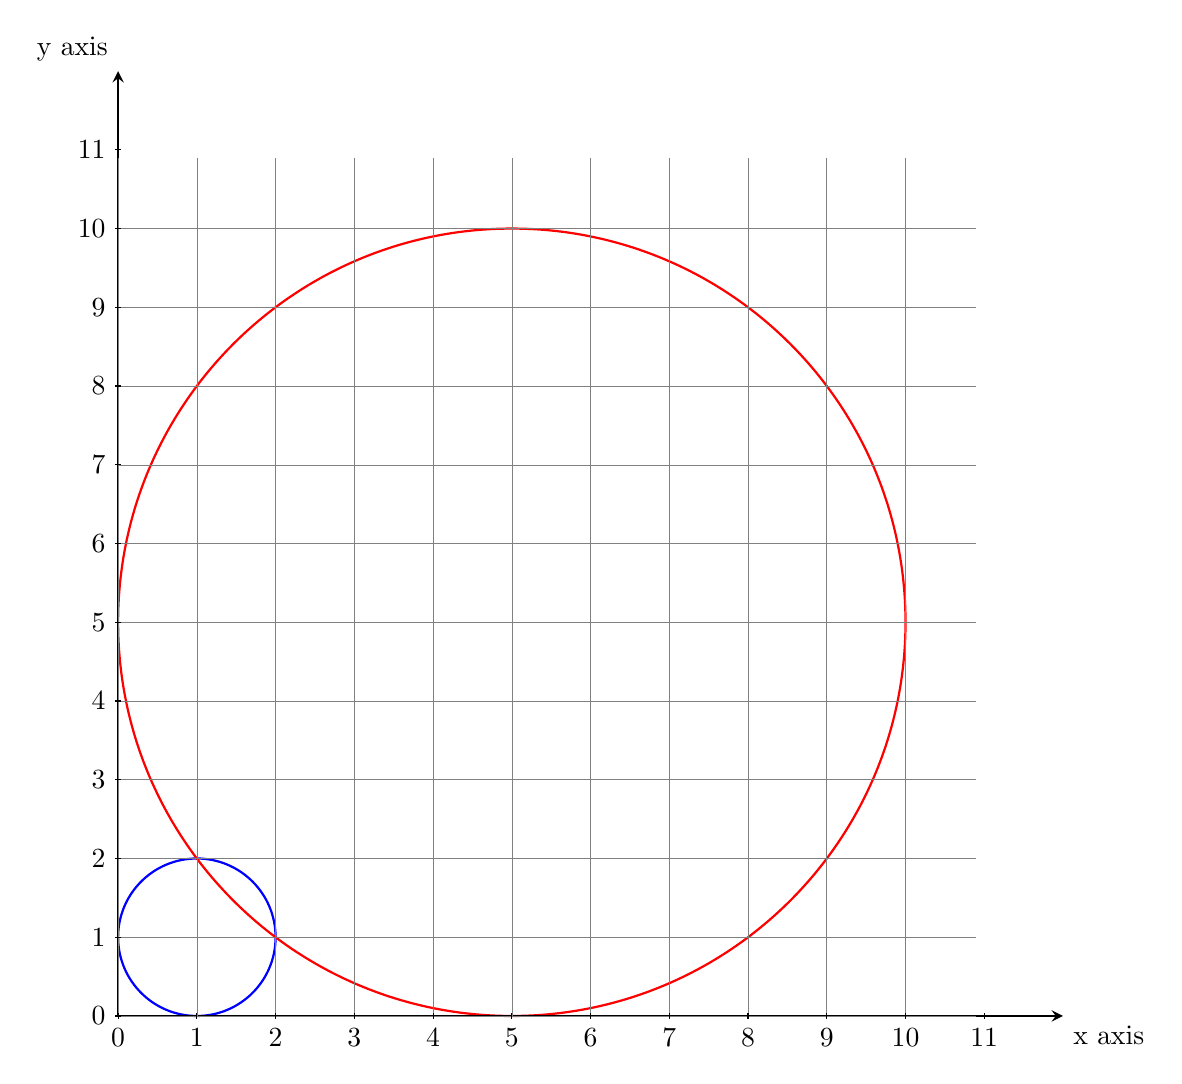
\begin{tikzpicture}
  [scale=1,>=stealth,point/.style={draw,circle,fill = black,inner sep=0.5pt},]
 
\draw [blue,thick,->](1,1) circle (1cm);
\draw [red,thick,->] (5,5) circle (5cm);
\draw[thick,->] (0,0) -- (12,0) node[anchor=north west] {x axis};
\draw[thick,->] (0,0) -- (0,12) node[anchor=south east] {y axis};
\draw[step=1cm,gray,very thin] (0,0) grid (10.9,10.9);

\foreach \x in {0,1,2,3,4,5,6,7,8,9,10,11}
\draw (\x cm,1pt) -- (\x cm,-1pt) node[anchor=north] {$\x$};
\foreach \y in {0,1,2,3,4,5,6,7,8,9,10,11}
\draw (1pt,\y cm) -- (-1pt,\y cm) node[anchor=east] {$\y$};

  \end{tikzpicture}
  	
